\documentclass[12pt,]{article}
\usepackage{lmodern}
\usepackage{amssymb,amsmath}
\usepackage{ifxetex,ifluatex}
\usepackage{fixltx2e} % provides \textsubscript
\ifnum 0\ifxetex 1\fi\ifluatex 1\fi=0 % if pdftex
  \usepackage[T1]{fontenc}
  \usepackage[utf8]{inputenc}
\else % if luatex or xelatex
  \ifxetex
    \usepackage{mathspec}
  \else
    \usepackage{fontspec}
  \fi
  \defaultfontfeatures{Ligatures=TeX,Scale=MatchLowercase}
\fi
% use upquote if available, for straight quotes in verbatim environments
\IfFileExists{upquote.sty}{\usepackage{upquote}}{}
% use microtype if available
\IfFileExists{microtype.sty}{%
\usepackage{microtype}
\UseMicrotypeSet[protrusion]{basicmath} % disable protrusion for tt fonts
}{}
\usepackage[margin=1in]{geometry}
\usepackage{hyperref}
\PassOptionsToPackage{usenames,dvipsnames}{color} % color is loaded by hyperref
\hypersetup{unicode=true,
            colorlinks=true,
            linkcolor=black,
            citecolor=Blue,
            urlcolor=black,
            breaklinks=true}
\urlstyle{same}  % don't use monospace font for urls
\usepackage{longtable,booktabs}
\usepackage{graphicx,grffile}
\makeatletter
\def\maxwidth{\ifdim\Gin@nat@width>\linewidth\linewidth\else\Gin@nat@width\fi}
\def\maxheight{\ifdim\Gin@nat@height>\textheight\textheight\else\Gin@nat@height\fi}
\makeatother
% Scale images if necessary, so that they will not overflow the page
% margins by default, and it is still possible to overwrite the defaults
% using explicit options in \includegraphics[width, height, ...]{}
\setkeys{Gin}{width=\maxwidth,height=\maxheight,keepaspectratio}
\IfFileExists{parskip.sty}{%
\usepackage{parskip}
}{% else
\setlength{\parindent}{0pt}
\setlength{\parskip}{6pt plus 2pt minus 1pt}
}
\setlength{\emergencystretch}{3em}  % prevent overfull lines
\providecommand{\tightlist}{%
  \setlength{\itemsep}{0pt}\setlength{\parskip}{0pt}}
\setcounter{secnumdepth}{0}

%%% Use protect on footnotes to avoid problems with footnotes in titles
\let\rmarkdownfootnote\footnote%
\def\footnote{\protect\rmarkdownfootnote}

%%% Change title format to be more compact
\usepackage{titling}

% Create subtitle command for use in maketitle
\newcommand{\subtitle}[1]{
  \posttitle{
    \begin{center}\large#1\end{center}
    }
}

\setlength{\droptitle}{-2em}
  \title{}
  \pretitle{\vspace{\droptitle}}
  \posttitle{}
  \author{}
  \preauthor{}\postauthor{}
  \date{}
  \predate{}\postdate{}

\usepackage{amsmath}
\usepackage{setspace}
\usepackage{rotating}
\usepackage[dvipsnames]{xcolor}
\usepackage{mathptmx}
\definecolor{mycol}{gray}{0}
\color{mycol}
\usepackage{enumitem}
\usepackage{wrapfig}
\usepackage[font={footnotesize,it}]{caption}
\usepackage{floatrow}
\usepackage{titlesec}
\titleformat{\section}{\normalfont\fontsize{14}{15}\bfseries}{\thesection}{1 em}{}
\titleformat{\subsection}{\normalfont\fontsize{12}{15}\bfseries}{\thesubsection}{1 em}{}
\titlespacing{\section}{0pt}{\parskip}{-\lineskip}
\titlespacing{\subsection}{0pt}{\parskip}{-\parskip}
\titlespacing{\subsubsection}{0pt}{\parskip}{-\parskip}
\newcounter{box}
\newcommand{\boxnumber}{\addtocounter{box}{1} \thebox \thinspace}
\floatstyle{boxed}
\newfloat{Box}{tbph}{box}

\begin{document}

\definecolor{blue}{rgb}{0,0,0.7}\newcommand{\new}{\textcolor{blue}}

\pagenumbering{roman}

\begin{description}
\item[Date:] \today
\item[Descriptive Title:] Synthesizing time series of plant and animal populations to understand the limits to ecological forecasts
\item[Short Title:] Ecological Forecasting
\item[PI Contact Information:] ~\\
\vspace{-1.5em}
\begin{description}
 \item[\textcolor{mycol}{Andrew Tredennick}] (atredenn@gmail.com; 970-443-1599) \\ Utah State University \\ 5230 Old Main Hill, Logan, UT 84332
 \item[\textcolor{mycol}{Mevin Hooten}] (Mevin.Hooten@colostate.edu) \\ U.S. Geological Survey \\ Colorado State University \\ Fort Collins, CO 80523
 \item[\textcolor{mycol}{Peter Adler}] (peter.adler@usu.edu) \\ Utah State University \\ 5230 Old Main Hill, Logan, UT 84332
\end{description}
\item[Project Summary:] Forecasting the impacts of global environmental change is a major challenge facing ecologists and land managers in the 21\textsuperscript{st} century. However, the potential to translate our deep understanding of ecological systems into skillful forecasts remains unknown. Emerging theory on partitioning forecast uncertainty provides an opportunity to evaluate the current limits to ecological forecasts. We propose to convene a diverse working group of quantitative ecologists, each with detailed knowledge of a particular study system, to develop forecasting models of plant and animal populations. As a team, we will partition the forecast uncertainty for each focal population to test fundamental hypotheses about the relationship between particular sources of uncertainty and population characteristics. We will develop a forecast repository and a synthetic database of population time series coupled with environmental covariates that will be ideal for teaching and research. We anticipate our work will (1) catalyze a new research agenda for ecology focused on identifying what currently limits ecological forecasts and (2) immediately inform ongoing efforts to monitor, model, and predict ecological dynamics.
\item[Proposed Start and End Dates:] January 2019 to December 2020, with two 4-day meetings at the Powell Center
\item[Proposed Data Release Date:] January 2021
\item[Total Requested Budget:] \$136,566 (Year 1 \$16,625; Year 2 \$118,141)
\item[Is this a resubmission?] Yes (first submission date: January 31, 2017)
\item[Conflicts of Interest with Reviewers:] None
\item[Keywords:] climate and land use change; ecosystems
\end{description}

\newpage{}

\pagenumbering{arabic}

\section{Problem Statement}

A fundamental challenge facing society is to predict the ecological
impacts of global environmental changes such as nitrogen deposition,
climate change, and habitat fragmentation. Each of these global change
drivers have now exceeded their historical ranges of variability
(Steffen et al. 2015), ushering in a no-analog era in which the past
cannot predict the future. We can, however, look to the past to
parameterize models that allow us to \emph{forecast} the future states
of ecological systems (Clark et al. 2001, Dietze et al. 2018).
Ecologists are in an excellent position to meet this forecasting
challenge because we have spent decades gaining understanding of the
processes that regulate populations, communities, and ecosystems.
However, we lack a systematic understanding of the current limits to
ecological forecasts. As a result, we do not know how to allocate
research effort to improve our forecasts.

Making poor forecasts is inevitable as ecology matures into a more
predictive science. The key is to learn from our failures so that
forecasts become more accurate over time. The success of meteorological
forecasting tells us that basic research on the causes of forecast
uncertainty is an essential component of this learning process (Bauer et
al. 2015).

Various approaches have been used to characterize and partition forecast
uncertainty (Sobol' 1993, Cariboni et al. 2007). For example, consider a
dynamic model designed to predict some state \emph{y} in the future
(\(y_{t+1}\)) based on the current state (\(y_{t}\)), an environmental
driver(s) (\(x\)), parameters (\(\theta\)), and process error
(\(\epsilon\)). We can then write a general form of the model as:
\begin{align}
y_{t+1} = f(y_t, x_t|\theta) + \epsilon_{t+1},
\end{align} which states that \(y\) at time \(t+1\) is a function of
\(y\) and \(x\) at time \(t\) conditional on the model parameters
(\(\theta\)) plus process error (\(\epsilon\)). Ignoring covariance
among factors, Dietze (2017), following Sobol' (1993) and Cariboni et
al. (2007), suggests that forecast variance (\(Var[y_{t+1}]\)) is
approximately: \begin{align}
Var[y_{t+1}] \approx \underbrace{\left(\frac{\delta f}{\delta y} \right)^2}_{\text{stability}} 
               \underbrace{\vphantom{ \left(\frac{\delta f}{\delta y} \right)^2 } Var[y_t]}_{\text{IC uncert.}} +
               \underbrace{\vphantom{ \left(\frac{\delta f}{\delta y} \right)^2 }\left(\frac{\delta f}{\delta x} \right)^2}_{\text{driver sens.}} 
               \underbrace{\vphantom{ \left(\frac{\delta f}{\delta y} \right)^2 } Var[x_t]}_{\text{driver uncert.}} +
               \underbrace{\vphantom{ \left(\frac{\delta f}{\delta y} \right)^2 }\left(\frac{\delta f}{\delta \theta} \right)^2}_{\text{param sens.}}
               \underbrace{\vphantom{ \left(\frac{\delta f}{\delta y} \right)^2 } Var[\theta]}_{\text{param. uncert.}} +
               \underbrace{\vphantom{ \left(\frac{\delta f}{\delta y} \right)^2 } Var[\epsilon_{t+1}]}_{\text{process error}},
\end{align}

where each additive term follows a pattern of \emph{sensitivity} times
\emph{variance} and ``IC uncert.'' refers to ``\emph{I}nitial
\emph{C}onditions uncertainty.'' The variance attributable to any
particular factor is a function of how sensitive the model is to the
factor and the variance of that factor. For example, the atmosphere is a
chaotic system, meaning its dynamics are internally unstable and
sensitive to initial conditions uncertainty. This is why billions of
dollars are spent each year to measure meterological variables --
meterologists learned that the key to reducing forecast error
\((Var[y_{t+1}])\) was to reduce the uncertainty of initial conditions
(\(Var[y_t]\)).

In contrast, ecologists are attempting to make actionable forecasts with
little knowledge of which term in Eq. 2 dominates forecast error.
Knowing which term dominates forecast error in different ecological
settings will advance our fundamental understanding of the natural world
and immediately impact practical efforts to monitor, model, and predict
ecological dynamics. While it is impossible to partition forecast
uncertainty for every species on Earth, links among the dominant source
of forecast error and species' life histories might serve as prior
information that can guide new monitoring and modeling efforts.

\textbf{\emph{The goal of this project is to synthesize forecasts of plant and animal populations to advance our fundamental knowledge of the current limits to ecological forecasts}}.
We will convene a diverse group of population ecologists to partition
forecast uncertainty for several species and systematically link sources
of uncertainty to characteristics of the focal populations (e.g., life
history traits). Doing so will (1) quantify the current limits to
ecological forecasts, (2) create a bridge between ecological theory and
ecological forecasts, and (3) provide actionable information on new ways
to improve ongoing ecological forecasts.

\section{Hypotheses}

All forecasts are uncertain, and reducing forecast uncertainty hinges
upon knowing the source of uncertainty. The premise of this proposal is
that ecological characteristics of organisms (e.g., life history) are
related to sources of forecast uncertainty. Specifically, we pose three
hypotheses motivated by recent reviews of ecological forecasting
(Petchey et al. 2015, Houlahan et al. 2017).

\begin{description}

\item[H1.] \textbf{The contribution of initial conditions uncertainty to forecast uncertainty is greater for fast growing populations than for slow growing populations.} Fast growing populations are more likely to exhibit chaotic or near-chaotic dynamics, which inflate forecast uncertainty due to initial conditions uncertainty. To test this hypothesis we will regress the proportion of uncertainty attributable to initial conditions against estimated intrinsic population growth rates.

\item[H2.] \textbf{The contribution of driver uncertainty to forecast uncertainty is greater for species that ``predict'' than for species that ``bet-hedge'' against environmental conditions.} In variable environments, annual plants have developed two strategies for maintaining fitness despite fluctuating conditions: (i) bet-hedging, where germination is low but constant, and (ii) predictive germination, where germination rates, cued by the environment, vary substantially from year to year. Bet-hedgers should be insensitive to environmental drivers, and thus to driver uncertainty. We will compare forecast partitions for winter annual plants that span a spectrum from bet-hedgers to predictors (Gremer et al. 2014) to test this hypothesis. To apply this approach to our other focal data sets, we will quantify interannual variation of vital rates to determine where species lie on the bet-hedging spectrum (e.g., Botero et al. 2015).

\item[H3.] \textbf{The contribution of process uncertainty to forecast uncertainty increases with the number of trophic links.} We are using single-species population models in which trophic interactions are implicit, not explicit. If trophic interactions are important our models will poorly represent the process. We will compare forecast partitions for all data sets to test this hypothesis. Our working group will consist of experts for each data set (Tables 1 and 2), enabling us to develop food webs for each focal species based on expert knowledge. 

\end{description}

Testing our hypotheses requires applying a standardized analytical
approach to a synthetic data set representative of many species -- an
activity that \emph{\textbf{can only be done at the Powell Center}} as a
working group.

\section{Proposed Activities}

PIs Tredennick, Hooten, and Adler have led several efforts to forecast
the response of plant populations to climate change (Tredennick et al.
2016, 2017). Our frustration with the high levels of uncertainty in our
forecasts, and our inability to attribute that uncertainty to specific
causes, has motivated this proposal. We seek to (1) assemble a database
of publicly available time series of plant and animal abundances which
contain the necessary data, (2) use those data to fit forecasting
models, and (3) partition the forecast uncertainty from those models to
better understand the limits to ecological forecasting. We have learned
that collating large data sets and rigorously fitting statistical
population models requires dedicated effort. We therefore request
funding for a Powell Fellow (to be recruited) to lead the proposed work.

\subsection{Data Synthesis}

We have identified 12 potential data sets (Table 1) and our working
group members (Table 2) may identify more based on their professional
networks. All abundance data sets will be combined into a single
database that can be queried using standard SQL software. The abundance
data will be linked to a second database of environmental covariates. We
will extract climate data as needed from gridded data products (e.g.,
PRISM). We will work with study area experts (Table 2) to decide on
appropriate climate covariates for each time series.

\footnotesize

\begin{longtable}[]{@{}llll@{}}
\caption{Publicly-available abundance time series for plants and
animals.}\tabularnewline
\toprule
Taxa & Species (common name) & Length (yrs.) &
Citation/Website\tabularnewline
\midrule
\endfirsthead
\toprule
Taxa & Species (common name) & Length (yrs.) &
Citation/Website\tabularnewline
\midrule
\endhead
Animal & \emph{Bison bison} (American Bison) & 35 & Hobbs et al.
(2015)\tabularnewline
Animal & \emph{Enhydra lutris} (Sea otter) & 20 & Williams et al.
(2017)\tabularnewline
Animal & Breeding birds* & 47 &
\url{http://www.pwrc.usgs.gov/bbs/}\tabularnewline
Animal & \emph{Dipodomys} spp. (Kangaroo rats)* & 39 & Ernest et al.
(2015)\tabularnewline
Animal & Grasshopper spp.* & 10 (weekly census) &
\url{http://ghopclimate.colorado.edu}\tabularnewline
Animal & Antarctic penguin spp.* & 38 &
\url{http://www.penguinmap.com/}\tabularnewline
Plant & Sagebrush steppe perennial plants* & 22 & Zachmann et al.
(2010)\tabularnewline
Plant & AZ desert annuals* & 14 & Ernest et al. (2015)\tabularnewline
Plant & \emph{Artemisia} spp. (Sagebrush spp.) & 27 & Homer et al.
(2013)\tabularnewline
Plant & Alpine tundra plants* & 11 &
\url{http://niwot.colorado.edu/}\tabularnewline
Plant & Winter annuals (Desert Lab LTREB)* & 30 & Gremer and Venable
(2014)\tabularnewline
Plant & Mt. St.~Helens plants* & 30 & del Moral (2010)\tabularnewline
\bottomrule
\end{longtable}

\vspace{-2em}

*These data sets contain observations for many species.

\normalsize

\subsection{Analysis}\subsubsection{Dynamic Forecasting Models}

Using the assembled time series, we will fit Bayesian hierarchical
state-space models, which are well-suited for ecological forecasting
because they incorporate and propagate the uncertainties we seek to
partition: process uncertainty, observation uncertainty, and parameter
uncertainty. State-space models also explicitly acknowledge that our
observations are imperfect, meaning that the state we want to estimate
(e.g., abundance of bison in Yellowston) is unknowable, or
\emph{latent}. A typical state-space model takes the form: \begin{align}
y_t &\sim \text{Normal}(z_t, \sigma^2_{\text{o}}), \\
z_t &\sim \text{Normal}\left(f(\boldsymbol{\theta},z_{t-1},\bold{x}_t), \sigma^2_{\text{p}}\right),
\end{align}

\begin{wrapfigure}[31]{tr}{0.45\textwidth}
  \centering
     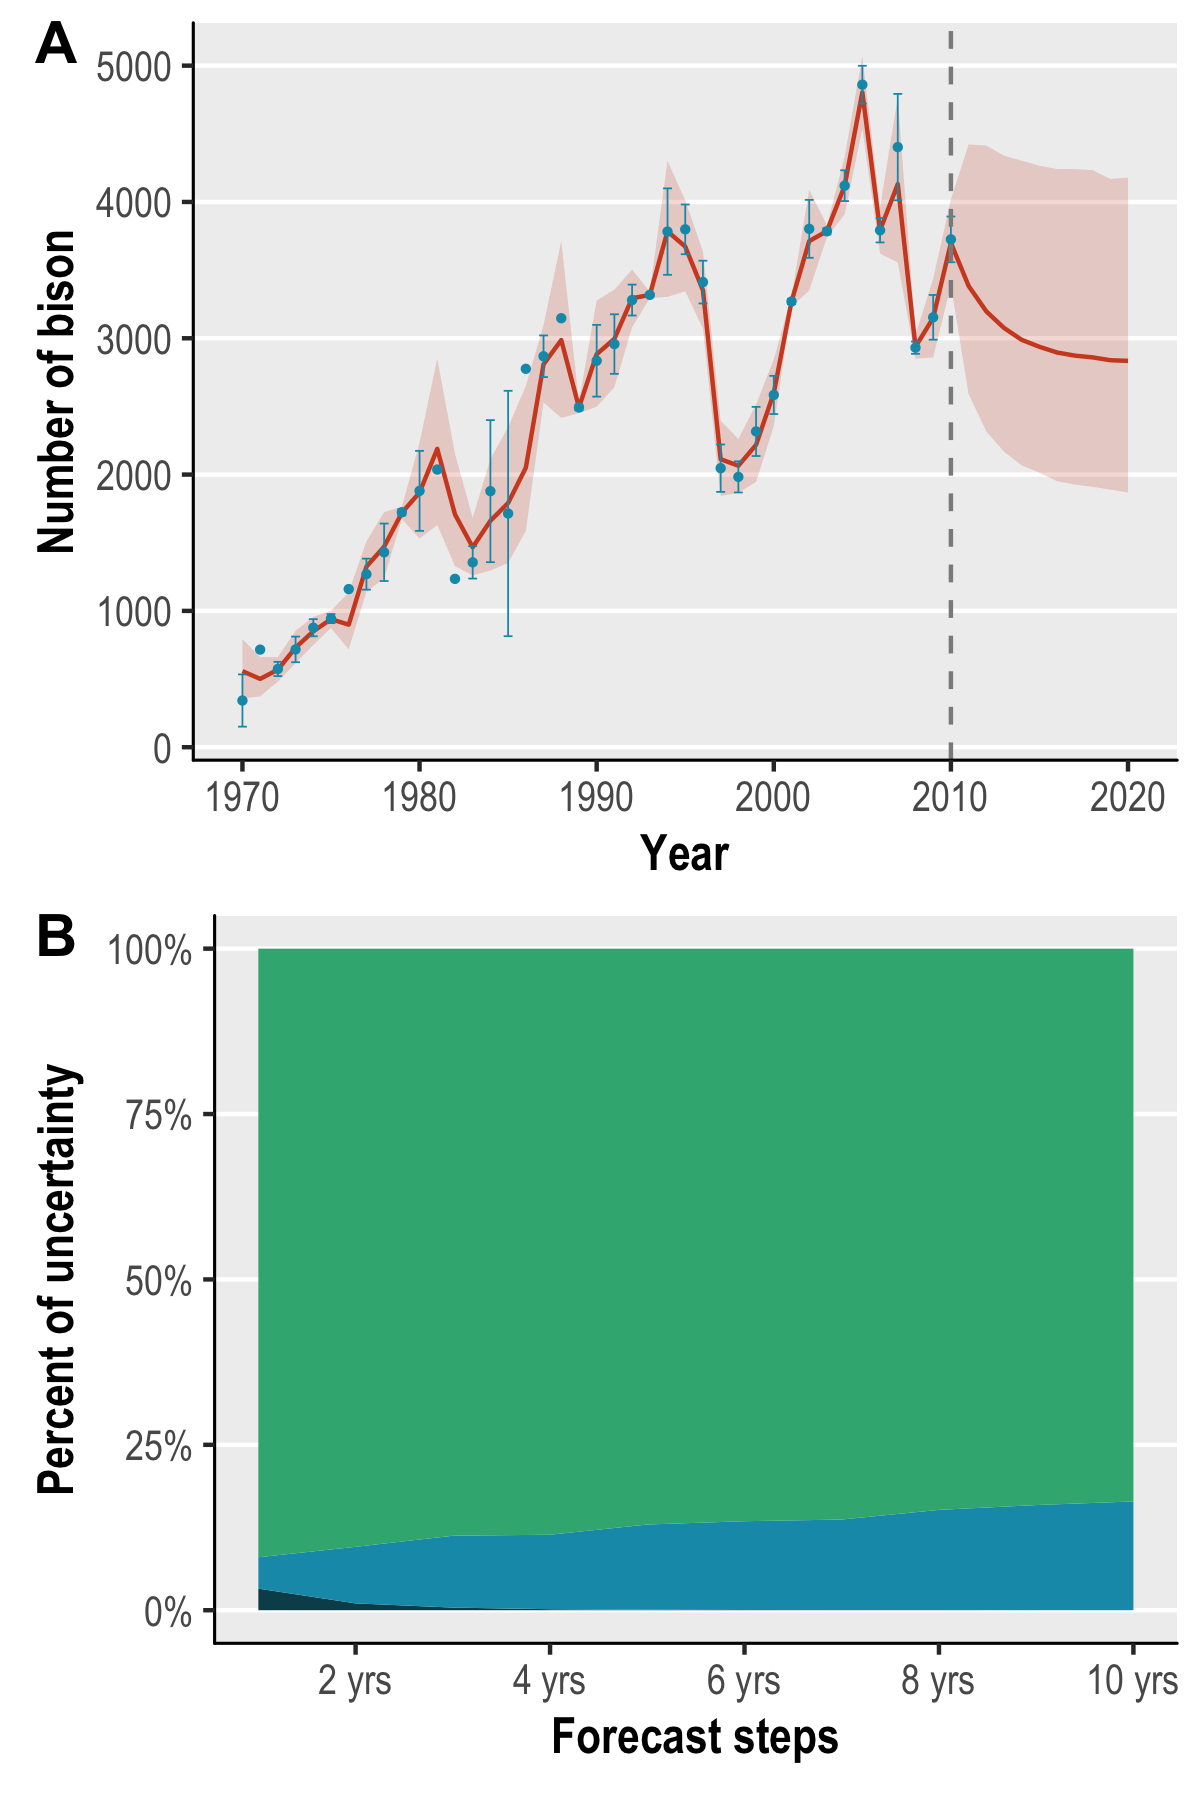
\includegraphics[height=4in]{../figures/bison_combined.png}
  \caption{An example state space model fit and forecast (A) and example of forecast uncertainty partitioning (B). In (A), points are observed counts and error bars show the observed standard deviation; solid line is the median of the posterior distribution of the number of bison in Yellowstone and shaded area shows the 95\% Bayesian Credible Interval. Within-sample estimates are constrained by data, whereas the forecasts (past 2010) are not. Panel (B) shows the relative contribution of each source of forecast uncertainty over time.}
\end{wrapfigure}

where \(y_t\) is the observed state at time \emph{t}, \(z_t\) is the
latent state at time \emph{t}, \(\mu_t\) is the determinstic prediction
of the state at time \emph{t} given estimated parameters
(\(\boldsymbol{\theta}\)) for the specified model function
{[}\emph{f()}{]}, the latent state \emph{z} at time \emph{t}-1, and
\(\textbf{x}_t\) is a vector of environmental covariates. The two error
terms represent observation error (\(\sigma^2_{\text{o}}\)) and process
error (\(\sigma^2_{\text{p}}\)). The model is \emph{dynamic} because the
future state (\(z_t\)) depends on the previous state (\(z_{t-1}\)). We
show the data and process models (Eqs. 3 and 4, respectively) with
normal likelihoods, but the distribution of the data model will vary
depending on the particular data generating process (Hobbs and Hooten
2015). Using different distributions for the data and process models
also helps make variance parameters identifiable when replicate
observations are not available (Hobbs and Hooten 2015), thus avoiding a
potential pitfall of state-space models (Auger-Méthé et al. 2016).

\subsubsection{An Example: Yellowstone Bison}

We used annual counts of the Yellowston bison from 1975 to 2010 to fit a
population growth model using a state-space approach. After fitting the
model, we made annual forecasts for 7 years into the future with all
uncertainty propagated (Fig. 1A). We made those same forecasts with
(\emph{i}) just initial condition uncertainty; (\emph{ii}) initial
condition and parameter uncertainty; (\emph{iii}) initial condition,
parameter, and driver uncertainty; and (\emph{iv}) initial condition,
parameter, driver, and process uncertainty. This set of forecasts allows
us to partition the relative uncertainty from different sources, taking
a numerical approach that is analagous to the analytical approach shown
in Equation 2.

The key result is that parameter uncertainty dominates forecast
uncertainty at all horizons, with a shift toward driver and process
error at later horizons (Fig. 1B). Initial condition uncertainty decays
very quickly, indicating strong internal population regulation and the
lack of chaotic dynamics, which is consistent with our
\textbf{Hypothesis H1}. A rigorous test of \textbf{H1} will require
comparison with results from fast-growing populations.

\section{Participants}

Our working group contains both gender and career stage diversity (Table
2). Of the 14 listed participants, five are women and six are early
career scientists. Several participants bring expert knowledge of a
particular dataset, some bring analytical experitise, and many bring
both. Participants will break into analysis teams, each responsible for
two or three datasets. Analysis teams will work together duing the
meetings at the Powell Center to develop a modeling framework for their
datasets, which will be presented back to the larger group for
discussion. The Powell Fellow will be responsible for implementing the
modeling approach, with significant contributions from analysis teams.

\footnotesize

\begin{longtable}[]{@{}llll@{}}
\caption{List of participants.}\tabularnewline
\toprule
\begin{minipage}[b]{0.22\columnwidth}\raggedright
Name\strut
\end{minipage} & \begin{minipage}[b]{0.22\columnwidth}\raggedright
Affiliation\strut
\end{minipage} & \begin{minipage}[b]{0.25\columnwidth}\raggedright
Expertise\strut
\end{minipage} & \begin{minipage}[b]{0.19\columnwidth}\raggedright
Associated Data set\strut
\end{minipage}\tabularnewline
\midrule
\endfirsthead
\toprule
\begin{minipage}[b]{0.22\columnwidth}\raggedright
Name\strut
\end{minipage} & \begin{minipage}[b]{0.22\columnwidth}\raggedright
Affiliation\strut
\end{minipage} & \begin{minipage}[b]{0.25\columnwidth}\raggedright
Expertise\strut
\end{minipage} & \begin{minipage}[b]{0.19\columnwidth}\raggedright
Associated Data set\strut
\end{minipage}\tabularnewline
\midrule
\endhead
\begin{minipage}[t]{0.22\columnwidth}\raggedright
Andrew Tredennick*\(^{1,2}\)\strut
\end{minipage} & \begin{minipage}[t]{0.22\columnwidth}\raggedright
Utah State University\\
\strut
\end{minipage} & \begin{minipage}[t]{0.25\columnwidth}\raggedright
Data management/synthesis,\\
population forecasting\strut
\end{minipage} & \begin{minipage}[t]{0.19\columnwidth}\raggedright
n/a\strut
\end{minipage}\tabularnewline
\begin{minipage}[t]{0.22\columnwidth}\raggedright
Mevin Hooten*\(^\dagger\)\strut
\end{minipage} & \begin{minipage}[t]{0.22\columnwidth}\raggedright
U.S. Geological Survey\\
\strut
\end{minipage} & \begin{minipage}[t]{0.25\columnwidth}\raggedright
Bayesian modeling,\\
statistical forecasting\strut
\end{minipage} & \begin{minipage}[t]{0.19\columnwidth}\raggedright
Sea otter\strut
\end{minipage}\tabularnewline
\begin{minipage}[t]{0.22\columnwidth}\raggedright
Peter Adler*\strut
\end{minipage} & \begin{minipage}[t]{0.22\columnwidth}\raggedright
Utah State University\\
\strut
\end{minipage} & \begin{minipage}[t]{0.25\columnwidth}\raggedright
population ecology/modeling,\\
data synthesis\strut
\end{minipage} & \begin{minipage}[t]{0.19\columnwidth}\raggedright
Idaho sagebrush\strut
\end{minipage}\tabularnewline
\begin{minipage}[t]{0.22\columnwidth}\raggedright
Lauren Buckley*\strut
\end{minipage} & \begin{minipage}[t]{0.22\columnwidth}\raggedright
University of Washington\\
\strut
\end{minipage} & \begin{minipage}[t]{0.25\columnwidth}\raggedright
ecological forecasting\\
climate change\strut
\end{minipage} & \begin{minipage}[t]{0.19\columnwidth}\raggedright
Grasshopper spp.\strut
\end{minipage}\tabularnewline
\begin{minipage}[t]{0.22\columnwidth}\raggedright
Michael Dietze*\strut
\end{minipage} & \begin{minipage}[t]{0.22\columnwidth}\raggedright
Boston University\\
\strut
\end{minipage} & \begin{minipage}[t]{0.25\columnwidth}\raggedright
ecological forecasting,\\
partitioning uncertainty\strut
\end{minipage} & \begin{minipage}[t]{0.19\columnwidth}\raggedright
n/a\strut
\end{minipage}\tabularnewline
\begin{minipage}[t]{0.22\columnwidth}\raggedright
George Esslinger*\strut
\end{minipage} & \begin{minipage}[t]{0.22\columnwidth}\raggedright
U.S. Geological Survey\\
Alaska Science Center\strut
\end{minipage} & \begin{minipage}[t]{0.25\columnwidth}\raggedright
population monitoring,\\
GIS analysis\strut
\end{minipage} & \begin{minipage}[t]{0.19\columnwidth}\raggedright
Sea otter\strut
\end{minipage}\tabularnewline
\begin{minipage}[t]{0.22\columnwidth}\raggedright
Emily Farrer*\strut
\end{minipage} & \begin{minipage}[t]{0.22\columnwidth}\raggedright
Tulane University\\
\strut
\end{minipage} & \begin{minipage}[t]{0.25\columnwidth}\raggedright
population modeling,\\
Bayesian analysis\strut
\end{minipage} & \begin{minipage}[t]{0.19\columnwidth}\raggedright
Niwot plants\strut
\end{minipage}\tabularnewline
\begin{minipage}[t]{0.22\columnwidth}\raggedright
Jennifer Gremer*\strut
\end{minipage} & \begin{minipage}[t]{0.22\columnwidth}\raggedright
University of California,\\
Davis\strut
\end{minipage} & \begin{minipage}[t]{0.25\columnwidth}\raggedright
plant population modeling\\
data management\strut
\end{minipage} & \begin{minipage}[t]{0.19\columnwidth}\raggedright
Winter annuals\strut
\end{minipage}\tabularnewline
\begin{minipage}[t]{0.22\columnwidth}\raggedright
Janneke HillRisLambers*\strut
\end{minipage} & \begin{minipage}[t]{0.22\columnwidth}\raggedright
University of Washington\strut
\end{minipage} & \begin{minipage}[t]{0.25\columnwidth}\raggedright
plant population modeling,\\
climate change\strut
\end{minipage} & \begin{minipage}[t]{0.19\columnwidth}\raggedright
Mt. St.~Helens plants\strut
\end{minipage}\tabularnewline
\begin{minipage}[t]{0.22\columnwidth}\raggedright
N. Thompson Hobbs*\(^\dagger\)\strut
\end{minipage} & \begin{minipage}[t]{0.22\columnwidth}\raggedright
Colorado State University\\
\strut
\end{minipage} & \begin{minipage}[t]{0.25\columnwidth}\raggedright
population ecology,\\
state space models\strut
\end{minipage} & \begin{minipage}[t]{0.19\columnwidth}\raggedright
Yellowstone bison\strut
\end{minipage}\tabularnewline
\begin{minipage}[t]{0.22\columnwidth}\raggedright
Heather Lynch*\strut
\end{minipage} & \begin{minipage}[t]{0.22\columnwidth}\raggedright
Stony Brook University\strut
\end{minipage} & \begin{minipage}[t]{0.25\columnwidth}\raggedright
population modeling,\\
population forecasting\strut
\end{minipage} & \begin{minipage}[t]{0.19\columnwidth}\raggedright
Antarctic penguins\strut
\end{minipage}\tabularnewline
\begin{minipage}[t]{0.22\columnwidth}\raggedright
Ethan White*\strut
\end{minipage} & \begin{minipage}[t]{0.22\columnwidth}\raggedright
University of Florida\\
\strut
\end{minipage} & \begin{minipage}[t]{0.25\columnwidth}\raggedright
ecological forecasting,\\
data synthesis\strut
\end{minipage} & \begin{minipage}[t]{0.19\columnwidth}\raggedright
BBS \& Portal Data\strut
\end{minipage}\tabularnewline
\begin{minipage}[t]{0.22\columnwidth}\raggedright
Perry Williams*\(^\dagger\)\strut
\end{minipage} & \begin{minipage}[t]{0.22\columnwidth}\raggedright
Colorado State University\\
\strut
\end{minipage} & \begin{minipage}[t]{0.25\columnwidth}\raggedright
spatiotemporal modeling,\\
population forecasts\strut
\end{minipage} & \begin{minipage}[t]{0.19\columnwidth}\raggedright
Sea otter\strut
\end{minipage}\tabularnewline
\begin{minipage}[t]{0.22\columnwidth}\raggedright
Postdoctoral Fellow\strut
\end{minipage} & \begin{minipage}[t]{0.22\columnwidth}\raggedright
TBD\\
\strut
\end{minipage} & \begin{minipage}[t]{0.25\columnwidth}\raggedright
population ecology,\\
population forecasts\strut
\end{minipage} & \begin{minipage}[t]{0.19\columnwidth}\raggedright
n/a\strut
\end{minipage}\tabularnewline
\bottomrule
\end{longtable}

\vspace{-2em}

*Confirmed participant; \(^\dagger\)Local (Ft. Collins) participant;
\(^1\)Technical liaison to Powell Center computing staff; \(^2\)Party
responsible for adherence to Powell Center Data and Information Policy

\normalsize

\section{Time Table of Activities}\begin{description}

\item[January to March 2019] Monthly PI Skype meetings to prepare for first meeting. Confirm participants. Write \texttt{R} scripts to download and clean data.
\item[April 2019] \textit{1st four day meeting at Powell Center}: Participants introduce their data sets. Decide on model structures for each data set and identify climate data availability. Form analysis teams. Define manuscripts.
\item[May 2019 to March 2020] Bi-monthly PI Skype meetings. Continue and finalize data set aquisition and aggregate into single database for analysis teams. Analysis teams, with the PC Fellow, identify appropriate climate drivers for their system and begin fitting state-space models. PC Fellow writes generalizable \texttt{R} functions for analysis teams. Write first drafts of manuscripts.
\item[April 2020] \textit{2nd four day meeting at Powell Center}: Analysis teams present results for feedback. Finalize database and identify any outstanding issues. Evaluate manuscript drafts and form writing teams. Create forecast repository.
\item[May to September 2020] Finalize database and forecast repository. Finalize all analyses. Continue writing manuscripts. PC Fellow works with analysis teams as needed.
\item[September to December 2020] Complete manuscripts and submit for publication. Release database and forecast repository to Powell Center for archiving.

\end{description}

\section{Anticipated Results and Benefits}

Ecological forecasts are central to ecosystem mangament, either
explicitly or implicitly.
\textbf{\emph{Understanding the sources of forecast error will provide actionable information that can guide management decisions by focusing data collection and model improvement efforts on areas that will most reduce forecast uncertainty}}
(Box 1). Another benefit of this project will be the conceptual advance
of linking ecological theory to sources of forecast uncertainty. We
anticipate that research associated with this project will catalyze a
new area of research on ecological forecasting. The working group
participants will gain experience using cutting-edge quantitative
techniques. The assembled database of plant and animal abundance time
series, coupled with environmental covariates, will be a valuable
resource for teaching and research, and the repository of population
forecasts will provide new opportunities to validate, and improve,
forecasts. In addition, we expect to produce several publications,
including:

\begin{enumerate}
\def\labelenumi{\arabic{enumi}.}
\tightlist
\item
  A synthesis paper testing our hypotheses using all the data sets aimed
  at \emph{PNAS} or \emph{Ecology Letters}.
\item
  A forum-style paper on the current limits to ecological forecasting,
  how to overcome them, and the usefulness of even uncertain forecasts
  for ecosystem management for \emph{Frontiers in Ecology and the
  Environment}.
\item
  Several in-depth papers on forecasts of specific populations aimed at
  top-tier applied journals such as \emph{Ecological Applications} and
  \emph{Journal of Applied Ecology}.
\end{enumerate}

\begin{Box}[!b]
  \renewcommand{\arraystretch}{1.04}
  \caption{Anticipated immediate and actionable outcomes of this working group.}
  \footnotesize
  \begin{description}
  \item[Inform priors] Linking forecast uncertainty to species' ecologies can allow researchers to use informed priors in Bayesian forecasting models, which can reduce parameter and process uncertainty.
  \item[Synergy] Contributes a large number of new case studies to ongoing efforts to assess the common patterns to ecological predictability across different processes and systems (e.g., the \emph{Near-term ecological forecasting initiative}).
  \item[Research and Development] Knowing the sources of uncertainty will allow us to determine whether more data, more precise data, or different modeling approaches will be most effective for improving our forecasts. It also lets us use scarce monitoring resources more efficiently by focusing efforts on where we will get the greatest return on investment in terms of reducing uncertainties in our predictions
  \item[Ecosystem Management] This working group will help improve existing population forecasts, which would immediately feed into advice to the management community.
  \end{description} 

  \renewcommand{\arraystretch}{1.0}
\end{Box}

\hypertarget{literature-cited}{%
\section*{Literature Cited}\label{literature-cited}}
\addcontentsline{toc}{section}{Literature Cited}

\hypertarget{refs}{}
\leavevmode\hypertarget{ref-Auger-Methe2016}{}%
Auger-Méthé, M., C. Field, C. M. Albertsen, A. E. Derocher, M. A. Lewis,
I. D. Jonsen, and J. M. Flemming. 2016. State-space models' dirty little
secrets: Even simple linear Gaussian models can have estimation
problems. Scientific Reports 6.

\leavevmode\hypertarget{ref-Bauer2015}{}%
Bauer, P., A. Thorpe, and G. Brunet. 2015. The quiet revolution of
numerical weather prediction. Nature 525:47--55.

\leavevmode\hypertarget{ref-Botero2015}{}%
Botero, C. A., F. J. Weissing, J. Wright, and D. R. Rubenstein. 2015.
Evolutionary tipping points in the capacity to adapt to environmental
change. Proceedings of the National Academy of Sciences 112:184--189.

\leavevmode\hypertarget{ref-Cariboni2007}{}%
Cariboni, J., D. Gatelli, R. Liska, and A. Saltelli. 2007. The role of
sensitivity analysis in ecological modelling. Ecological Modelling
203:167--182.

\leavevmode\hypertarget{ref-Clark2001}{}%
Clark, J. S., S. R. Carpenter, M. Barber, S. Collins, A. Dobson, J. A.
Foley, D. M. Lodge, M. Pascual, R. Pielke, W. Pizer, C. Pringle, W. V.
Reid, K. A. Rose, O. Sala, W. H. Schlesinger, D. H. Wall, and D. Wear.
2001. Ecological forecasts: an emerging imperative. Science
293:657--660.

\leavevmode\hypertarget{ref-DelMoral2010}{}%
del Moral, R. 2010. Thirty years of permanent vegetation plots, Mount
St. Helens, Washington, USA. Ecology 91:2185.

\leavevmode\hypertarget{ref-Dietze2017a}{}%
Dietze, M. C. 2017. Prediction in ecology: A first-principles framework.
Ecological Applications 27:2048--2060.

\leavevmode\hypertarget{ref-Dietze2018}{}%
Dietze, M., A. Fox, L. Beck-Johnson, J. Betancourt, M. Hooten, C.
Jarnevitch, T. Kiett, M. Kenney, C. Laney, L. Larsen, L. Loescher, C.
Lunch, P. Pijanowski, J. Randerson, E. Reid, A. T. Tredennick, R.
Vargas, K. Weathers, and E. P. White. 2018. Iterative near-term
ecological forecasting: Needs, opportunities, and challenges.
Proceedings of the National Academy of Sciences.

\leavevmode\hypertarget{ref-Gremer2014}{}%
Gremer, J. R., and D. L. Venable. 2014. Bet hedging in desert winter
annual plants: Optimal germination strategies in a variable environment.
Ecology Letters 17:380--387.

\leavevmode\hypertarget{ref-Hobbs2015}{}%
Hobbs, N. T., and M. B. Hooten. 2015. Bayesian Models: A Statistical
Primer for Ecologists. Princeton University Press, Princeton.

\leavevmode\hypertarget{ref-Houlahan2017}{}%
Houlahan, J. E., S. T. Mckinney, T. M. Anderson, and B. J. Mcgill. 2017.
The priority of prediction in ecological understanding. Oikos 126:1--7.

\leavevmode\hypertarget{ref-Petchey2015}{}%
Petchey, O. L., M. Pontarp, T. M. Massie, S. Kéfi, A. Ozgul, M.
Weilenmann, G. M. Palamara, F. Altermatt, B. Matthews, J. M. Levine, D.
Z. Childs, B. J. McGill, M. E. Schaepman, B. Schmid, P. Spaak, A. P.
Beckerman, F. Pennekamp, and I. S. Pearse. 2015. The ecological forecast
horizon, and examples of its uses and determinants. Ecology Letters
18:597--611.

\leavevmode\hypertarget{ref-Sobol1993}{}%
Sobol', I. 1993. Sensitivity Estimates for Nonlinear Mathematical
Models.

\leavevmode\hypertarget{ref-Steffen2015}{}%
Steffen, W., K. Richardson, J. Rockström, S. Cornell, I. Fetzer, E.
Bennett, R. Biggs, and S. Carpenter. 2015. Planetary boundaries: Guiding
human development on a changing planet. Science 348:1217.

\leavevmode\hypertarget{ref-Tredennick2016Ecos}{}%
Tredennick, A. T., M. B. Hooten, C. L. Aldridge, C. G. Homer, A. R.
Kleinhesselink, and P. B. Adler. 2016. Forecasting climate change
impacts on plant populations over large spatial extents. Ecosphere
7:e01525.

\leavevmode\hypertarget{ref-Tredennick2017a}{}%
Tredennick, A. T., M. B. Hooten, and P. B. Adler. 2017. Do we need
demographic data to forecast plant population dynamics? Methods in
Ecology and Evolution 8:541--551.

\leavevmode\hypertarget{ref-Williams2017a}{}%
Williams, P. J., M. B. Hooten, J. N. Womble, G. G. Esslinger, M. R.
Bower, and T. J. Hefley. 2017. An integrated data model to estimate
spatiotemporal occupancy, abundance, and colonization dynamics. Ecology
98:328--336.


\end{document}
